%%
% Name: IMS - Vodovody a kanalizace Vyškov
% Autors: Michal Cupak, Ales Dujicek
% Date: 2012-12-07
%%

%\documentclass[11pt,a4paper]{article}
\documentclass[12pt,a4paper]{article}
\usepackage[a4paper]{geometry}
\usepackage[czech]{babel}
%\usepackage{czech}
%\usepackage[latin2]{inputenc}
%\usepackage[IL2]{fontenc}
\usepackage[utf8]{inputenc}
%\usepackage[T1]{fontenc}
\usepackage{times}

\usepackage{graphics}
\usepackage{picture}
%\usepackage[czech,ruled]{algorithm2e}

\usepackage{amsmath}
\usepackage{amsthm}
\usepackage{amsfonts}

\usepackage{parskip}

%\newcommand{\uvoz}[1]{\quotedblbase #1\textquotedblleft}

\begin{document}

% Úvodní strana
%%
% Name: Titulní strana
% Autor: Michal Cupak
% Date: 2011-3-11
%%


\begin{titlepage}

\begin{center}
  
		{\Huge  {\scshape Vysoké učení technické v Brně}\\}
		{\huge {\scshape Fakulta informačních technologií}\\}
	
	\vspace{\stretch{0.382}}
		
	{\LARGE Modelování a simulace}
	\\
	\medskip
	{\Huge Vodovody a kanalizace Vyškov}\\
	\vspace{\stretch{0.618}}
\end{center}
{\Large \today \\\\ Michal Cupák \\ Aleš Dujíček}


\end{titlepage}


% Obsah
% \thispagestyle{empty}
% \tableofcontents
% \newpage

% Kapitola 1 - Úvod
\section{Úvod}
V této práci je řešena implementace systému hromadné obsluhy, která bude použita pro 
sestavení modelu zpracování dokumentů v administrativě firmy Vodovody a kanalizace Vyškov.

Na základě modelu a simulačních experimentů bude ukázáno 
chování systému toku dokumentů mezi jednotlivými zaměstnanci firmy v podmínkách běžné denní činnosti firmy.

Smyslem experimentů je demonstrovat, jak se při změně jakékoliv veličiny ovlivňující tok dokumentů ve studované firmě změní délka zpracování daného dokumentu či vy\-tí\-že\-ní ostatních zaměstnanců studované firmy.

Správnost zvolené koncepce byla ověřena přímo se zaměstnancem studované firmy.

\textit{(pro zpracování modelu bylo nutno nastudovat ..., zpracovat, ... model je ve svém oboru zajímavý/ojedinělý v ...)}

\subsection{Kdo se na práci podílel}
Autory této práce jsou studenti Fakulty informačních technologií Vysokého učení technického v Brně. Jmenovitě to jsou pánové Michal Cupák a Aleš Dujíček.

Fakta o společnosti nám laskavě poskytl pan Ing. Oldřich Novoměstský, vedoucí technického úseku společnosti Vodovody a kanalizace Vyškov.

Odborným konzultantem byl taktéž Ing. Novoměstský ve spolupráci s paní Annou Sý\-ko\-ro\-vou, se\-kre\-tář\-kou ředitele.

\subsection{Ověření validity modelu}
Ověřování validity modelu probíhalo při osobních setkáních s Ing. Novoměstským. Jednalo se především o vysvětlení problematiky zpracování dokumentů ve studované firmě. Dále pak o ověření funkčnosti modelu pomocí konzultace grafů vzniklých ze simulace.

Počet a procentuální rozdělení příchozích dokumentů byl konzultován s paní Sýkorovou, která má tyto dokumenty zpočátku na starosti.

\newpage


% Kapitola 2 - 
\section{Rozbor tématu a použitých metod/technologií}

Administrativa společnosti Vodovody a kanalizace Vyškov zahrnuje zpracování dokumentů (stížnosti, žádosti, smlouvy a dotazy), které jim lidé posílají poštou, elektronicky emaily a datovými schránkami a doručují osobně. Tok dokumentů je znázorněn na obrázku \ref{tok_dokumentu}.

Všechny příchozí dokumenty zpracovává sekretářka ředitele, která je musí naskenovat speciálním skenerem, vytisknout označené čárovým kódem a zaevidovat do informačního systému. Sekretářka se administrativní činnosti věnuje celou svou pracovní dobu.

Takto zpracované dokumenty prohlíží ředitel, který je dle obsahu či adresáta při\-dě\-lu\-je k vyřízení pracovníkům některému z úseků (úsek ředitele, ekonomický úsek, technický úsek). Ředitel se pro své vytížení jinými pracovními povinnostmi věnuje této administrativě průmerně hodinu denně.

V úseku ředitele jsou dokumenty přímo přidělovány ředitelem konkrétním pra\-cov\-ní\-kům.

Dokumenty k vyřízení v ekonomickém úseku prostuduje Ekonomický náměstek, který potom jejich vyřízením pověřuje své přímé podřízené.

% jeste tam je vedouci technickoho useku
V Technickém úseku dokumenty nejprve prostuduje Technický náměstek. Ten může jejich vyřízením pověřit své přímé podřízené, nebo může daný dokument předat Vedoucímu technického úseku, který jej následně předá k vyřízení některému ze dvých přímých podřízených.

Průměrně jednou až dvakrát měsíčně se objeví porucha technického zařízení, se kterým pracuje sekretářka. Ta potom po dobu opravy, která trvá průměrně 3 hodiny, nemůže dokumenty zpracovávat.

Pracovní doba zaměstnanců společnosti je 7,5 hodiny denně. Poštu přiváží pracovník pošty každý den mezi 9. a 10. hodinou, současně odveze odchozí poštu.

Denně je průmerně zaevidováno 50-60 příchozích dokumentů, které nejčastěji při\-chá\-zí klasickou poštou (20-30), dále elektronicky (20) a nejméně osobně (10).

Všechny informace uvedené v této kapitole byly poskytnuty zaměstnancem vedení společnosti, panem Ing. Oldřichem Novoměstským.

\begin{figure}[ht]
 \begin{center}
	\scalebox{0.68}{ 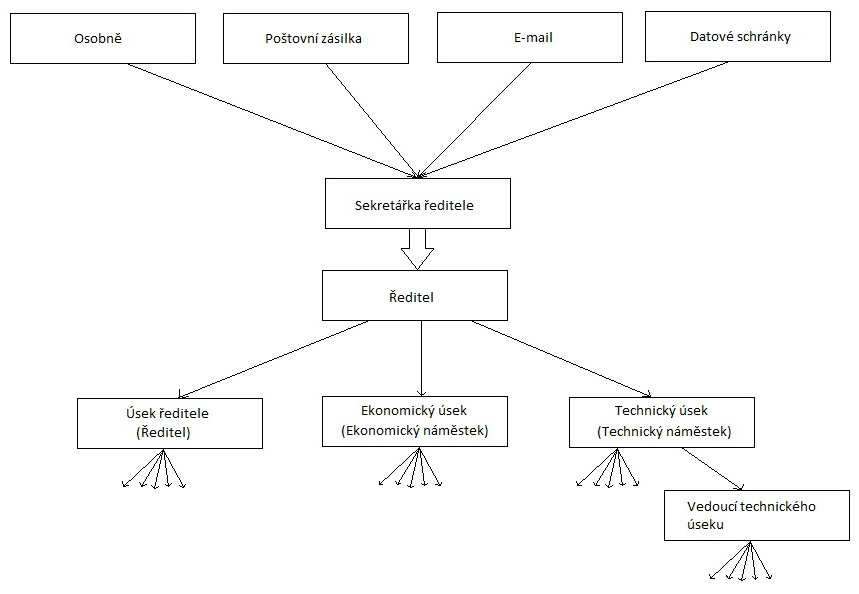
\includegraphics{tok_dokumentu.jpg} }
	\caption{Tok dokumentů v administrativě}
	\label{tok_dokumentu}
 \end{center}
\end{figure}

\subsection{Popis použitých postupů}
\subsection{Popis původu použitých metod}

\newpage

% Kapitola 3 - 
\section{Koncepce - modelářská témata}

Jako jednotku času v simulaci jsme zvolili jednu hodinu.
Modelovat budeme pouze pracovní dobu zaměstnanců. Noci, víkendy a jiné události, kvůli kterým se nepracuje, jsou vynechány.
Tedy v čase 0 začíná první pracovní den a v čase 7.5 začíná druhý bez ohledu na to, zda mezi nimi byl např. víkend.

Příchody dokumentů do systému modelujeme procesy zvlášť pro příchozí klasickou poštu, elekteronickou poštu a příchody lidí osobně.
Elektronická pošta zahrnuje emaily společně s datovými schránkami, není potřeba je rozlišovat, protože jejich zpracování probíhá totožně.
Příchody lidí jsou modelovány příchody procesů v intervalech daných exponenciálním rodělením se středem $T/n$, kde $T$ je délka pracovního dne v hodinách a $n$ průměrný počet příchodů denně.
Obdobně je modelován příchod dokumentů elektronicky, možnost příchodu elektronické zprvávy mimo pracovní dobu (např. v noci) zanedbáváme.

Ředitel společnosti je modelován zařízením s výlučným přístupem, které je po dobu 6.5 hodiny obsazeno procesem s prioritou obsluhy
představujícím všechny jeho pracovní povinnosti mimo administrativu, pro kterou je po zbylou 1 hodinu uvolněn.
Nezabýváme se, kdy přesně se administrativě ředitel věnuje, modelujeme pouze fakt, že se této činnosti věnuje pravidelně každý den danou dobu.
+ někdy je pryč pořád

další zpracování

poruchy

% Konceptuální model je abstrakce reality a redukce reality na soubor relevantních faktů pro sestavení simulačního modelu.
% Pokud některé partie reality zanedbáváte nebo zjednodušujete, musí to být zdůvodněno a videálním případě musí být prokázáno, že to neovlivní validitu modelu.
% Výsledek kapitoly: konceptuální (abstraktní) model s vyznačením relevantních faktů.

%  převzetí faktů do modelu
%  zdůvodněné provedené zjednodušení faktů
%  abstraktní popis modelu/programu

% Návod: koncepci vaší práce MUSÍ pochopit libovolný technik (a často i manažer...)

\newpage


% Kapitola 4 - 
\section{Architektura simulačního modelu/simulátoru}

% Nejméně zajímavá část. Obvykle se neuvádí.
% Rozeberte několik nejzajímavějších partií implementace
% Případná uživatelská příručka (spuštění programu, struktura výpisů, ...).
% O funkčnosti modelu musí přesvědčit kapitla 3.
% Není to referenční příručka!

% tuhle kapitolu asi hodne odflaknem, kdyz pise, ze neni zajimava
\newpage


% Kapitola 5 - 
\section{Podstata simulačních experimentů a jejich průběh}

% Experimentování musí mít předem zvolený a zdůvodněný řád, či postup
% 5.1 Postup experimentování a okolnosti studie
% 5.2 Dokumentace jednotlivých experimentů
% 5.3 Závěr experimentů
% Co bylo experimentováním zjištěno
% Jaké chyby v modelu byly odstraněny (oproti původním předpokladům ... došlo ke změně koncepce ... protože ..
\newpage


% Kapitola 6 - 
\section{Shrnutí simulačních experimentů a závěr}

% Jednoznačná odpověď na prvotní otázku studie.
%  Studií provedenou na našem modelu bylo jednoznačně prokázáno/vyvráceno, že ...
%  V rámci experimentů bylo zjištěno, že průměrné zatížení ... je ...
%  Z experimentů vyplývá jednoznačné doporučení, aby provozovatel ... rozšířil výrobu o ...
%  Ze statisticky zpracovaného měření v terénu plyne, že proces příchodů ... se řídí normálním rozložením se středem a ....
% • Na přiložených demo-příkladech jsme ověřili funkčnost ...

\newpage


\end{document}

